\documentclass{scrartcl}
\usepackage{amssymb}
\usepackage{amsmath}
\usepackage{tikz}
\usetikzlibrary{calc,intersections,through,backgrounds,patterns}
\usetikzlibrary{decorations.markings}
\usepackage{textcomp}

\begin{document}

%\begin{figure}
%	\centering
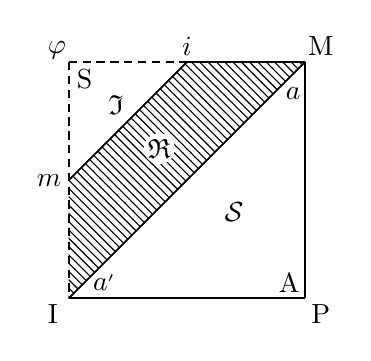
\begin{tikzpicture}

\coordinate (p) at (0,3) {};
\coordinate (M) at (3,3) {};
\coordinate (I) at (0,0) {};
\coordinate (P) at (3,0) {};
%
\coordinate (m) at (0,1.5) {};
\coordinate (i) at (1.5,3) {};

%outer lines
\draw [semithick, densely dashed]	(p)--(i); 	 %p--I
\draw [semithick]					(i)--(M); 	 %p--I
\draw [semithick, densely dashed]	(p)--(I);	 %p--I
\draw [semithick] 					(I)--(P);	 %I--P
\draw [semithick]  					(M)--(P);	 %M--P
%
\draw [semithick]  					(M)--(I); 	 %M--I
\draw [semithick]  					(m)--(i); 	 %m--i

\draw[pattern=north west lines, pattern color=black] (m)--(i)--(M)--(I);

%labels
\node at (-0.15,3.15)  {$\varphi$};
\node at (3.2,3.2)   {M};
\node at (-0.2,-0.2) {I};
\node at (3.2,-0.2)  {P};
%
\node at (-0.25,1.5) {$m$};
\node at (1.5,3.2)  {$i$};
%
\node at (2.8,0.2)  {A};
\node at (0.2,2.78) {S};
\node at (0.45,0.2) {$a${\scriptsize $^\prime$}};
\node at (2.85,2.6) {$a$};
%
\node at (2.1,1.1)  {$\mathcal{S}$};
\node at (0.6,2.45) {$\mathfrak{I}$};
%\node at (1.15,1.9) {$\mathfrak{R}$};
\node[circle,draw=white, fill=white, inner sep=0pt,minimum size=8pt] (R) at (1.15,1.9) {$\mathfrak{R}$};

\end{tikzpicture}
%	\caption{Lacan's Schema R}
%\end{figure}

\vspace{1cm}

%\begin{figure}
%	\centering
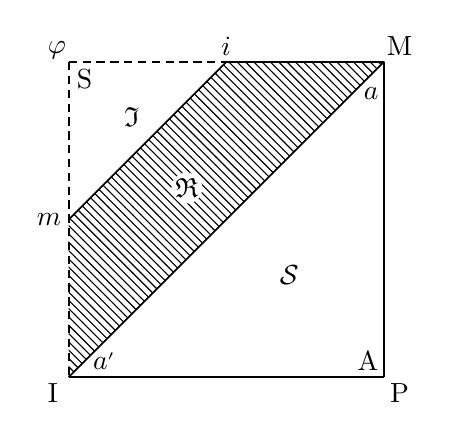
\begin{tikzpicture}

\coordinate (p) at (0,4) {};
\coordinate (M) at (4,4) {};
\coordinate (I) at (0,0) {};
\coordinate (P) at (4,0) {};
%
\coordinate (m) at (0,2) {};
\coordinate (i) at (2,4) {};

%outer lines
\draw [semithick, densely dashed]	(p)--(i); 	 %p--I
\draw [semithick]					(i)--(M); 	 %p--I
\draw [semithick, densely dashed]	(p)--(I);	 %p--I
\draw [semithick] 					(I)--(P);	 %I--P
\draw [semithick]  					(M)--(P);	 %M--P
%
\draw [semithick]  					(M)--(I); 	 %M--I
\draw [semithick]  					(m)--(i); 	 %m--i

\draw[pattern=north west lines, pattern color=black] (m)--(i)--(M)--(I);

%labels
\node at (-0.15,4.15)  {$\varphi$};
\node at (4.2,4.2)   {M};
\node at (-0.2,-0.2) {I};
\node at (4.2,-0.2)  {P};
%
\node at (-0.25,2) {$m$};
\node at (2,4.2)  {$i$};
%
\node at (3.8,0.2)  {A};
\node at (0.2,3.78) {S};
\node at (0.45,0.2) {$a${\scriptsize $^\prime$}};
\node at (3.84,3.6) {$a$};
%
\node at (2.8,1.3)  {$\mathcal{S}$};
\node at (0.8,3.3) {$\mathfrak{I}$};
\node[circle,draw=white, fill=white, inner sep=0pt,minimum size=8pt] (R) at (1.5,2.4) {$\mathfrak{R}$};

\end{tikzpicture}
%	\caption{Lacan's Schema R}
%\end{figure}

\end{document}